\begin{titlepage}
\newgeometry{top=1cm, left=3cm, right=3cm}
\begin{tabular}{lcr}
  \hspace{10cm} &
  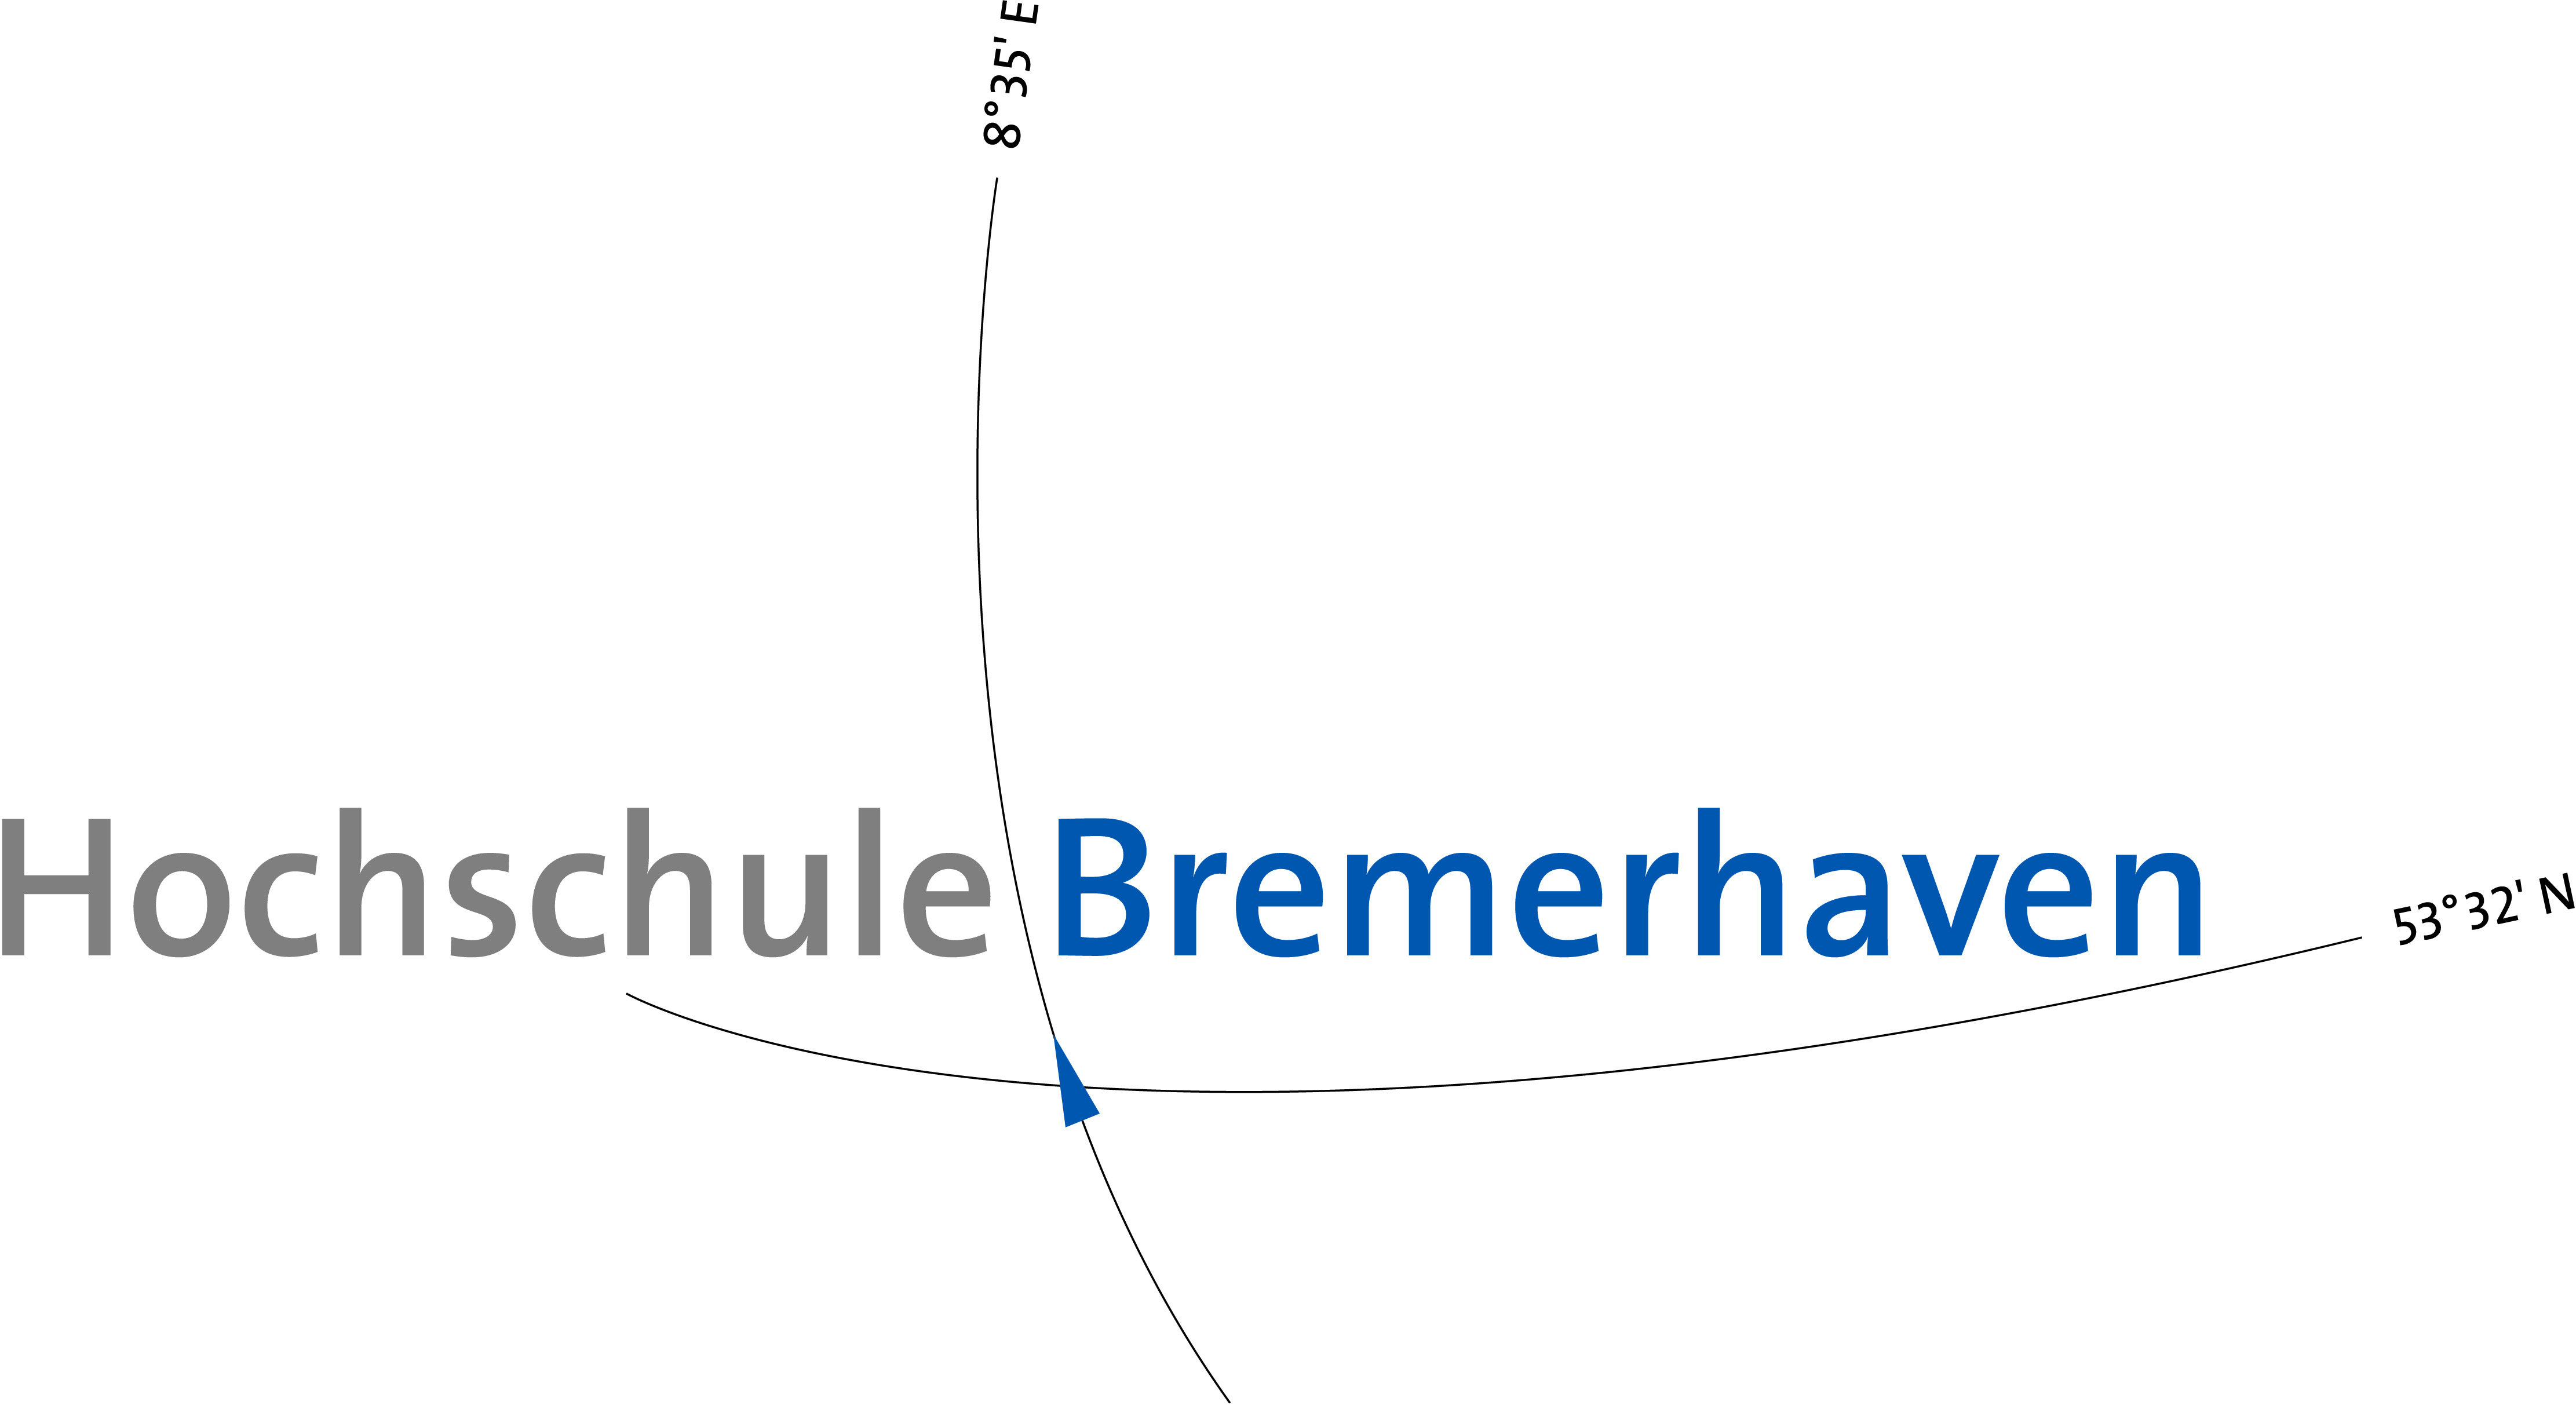
\includegraphics[width=170px]{images/hb_logo_2c.jpg}
  \vspace{1cm}
\end{tabular}
	\centering	
	\vspace{0cm}
	{\scshape\Large Digitalization, Innovation and Information Management \par}
	\vspace{1.5cm}
	{\Large\bfseries Master Thesis\par}
	\centering
    \vspace{2cm}
    {\Large\bfseries 
      Learning Representative Vessel Trajectories       Using  \par Deep Reinforcement Learning   \par
}
       {\normalsize\itshape
  Extracting Normality from AIS Data to Identify Anomalous Ship Behaviour
      \par}
	\vfill
	\vspace{2cm}
	\begin{tabularx}{\textwidth}{lX}
		Author: & Jan Löwenstrom (34937)\\
		Supervisors: & Prof. Dr.-Ing. Henrik Lipskoch \\ &(\textit{University of Applied Science Bremerhaven}) \\
		& Ph.D. Edgardo Solano Carrillo \\&(\textit{German Aerospace Center - Institute for the Protection of Maritime Infrastructures}, Bremerhaven)
		        
	\end{tabularx}  
    \vfill

% Bottom of the page with current date
	{\large \today \par}       
\end{titlepage}
\restoregeometry